\documentclass[10pt,twocolumn,letterpaper]{article}

\usepackage[margin=0.72in]{geometry}
\usepackage{amsmath,amssymb,amsfonts,amsthm}
\usepackage{booktabs}
\usepackage{graphicx}
\usepackage{hyperref}
\usepackage{microtype}
\usepackage{xcolor}
\usepackage{subcaption}

\hypersetup{
    colorlinks=true,
    linkcolor=blue!70!black,
    citecolor=blue!70!black,
    urlcolor=blue!70!black
}

\title{\textbf{Latent-Play: Sample-Efficient Goal Planning and Zero-Shot Physical Reasoning via Action-Free Video Pretraining and Isotropic JEPA World Models}}

\author{
  \textbf{Pedro Rivas Vega} \\
  \texttt{rivasvegap@gmail.com} \\
  \href{https://github.com/rivas-vega/latent-play}{\texttt{github.com/rivas-vega/latent-play}}
}

\date{October 2026}

\begin{document}

\maketitle

\begin{abstract}
Learning controllable world models from passive video without action labels is a central challenge for scaling embodied intelligence. While generative video models operate in pixel space with high sampling latency, Joint Embedding Predictive Architectures (JEPAs) predict directly in abstract representation space, yet face two fundamental obstacles: catastrophic representation collapse and reliance on ground-truth action labels that often suffer from visual aliasing (e.g., blocked movements or context-dependent no-ops). In this work, we present \textbf{latent-play}, an end-to-end framework that learns playable world models from unlabelled gameplay video. Our architecture couples: (i) a causal Spatio-Temporal Transformer with a motion-weighted, entropy-regularized Vector Quantized (VQ) bottleneck ($K=8$) to infer discrete latent actions without action supervision; (ii) an action-conditioned ViT-JEPA dynamics model regularized against dimensional collapse via the Statistical Invariant Geometric Regularizer (\textbf{SIGReg}), utilizing the Cram\'er-Wold device and differentiable Epps-Pulley characteristic function testing; and (iii) a receding-horizon Cross-Entropy Method (CEM) planner operating in representation space via a lightweight prior-corrected alignment probe. Evaluated on both a controlled \textbf{ToyGridEnv} ($100\text{K}$ frames) and the open-ended \textbf{Crafter} benchmark ($300\text{K}$ frames, $30\text{K}$ training steps on an NVIDIA A100), we demonstrate that: (1) discovered latent actions achieve $+10.05\text{ dB}$ controllability ($\Delta\text{PSNR}_{\text{ctrl}}$) with $100\%$ codebook utilization ($8/8$ codes); (2) conditioning JEPA dynamics on realized visual latent actions reduces 8-step rollout error by \textbf{24.0\% on Crafter} ($0.1523$ vs.\ $0.2003$) and 4-step error by \textbf{38.3\% on ToyGridEnv} ($0.1416$ vs.\ $0.2297$) compared to an oracle trained with ground-truth actions; (3) with only $0.1\%\text{--}10\%$ action labels, \textbf{latent-play} matches or exceeds the $100\%$-supervised action oracle in goal-directed CEM navigation ($28.0\%$ mean / $36.0\%$ peak on ToyGridEnv; $15.6\%$ mean / $26.7\%$ peak on Crafter vs.\ $10.0\%$ Oracle); and (4) the learned world model exhibits zero-shot physical Violation-of-Expectation (VoE) detection with surprise ratios of \textbf{15.25$\times$ on spatial teleportation} and \textbf{52.91$\times$ on object disappearance}.
\end{abstract}

\section{Introduction}
Foundation models in vision and language learn generalizable representations from passive web data. In embodied and spatial AI, however, policy and world model learning have traditionally required synchronized action logs. While billions of hours of gameplay and physical interaction video exist online, less than $0.01\%$ contain ground-truth controller trajectories.

Recent works such as Google DeepMind's Genie \cite{bruce2024genie} and LAPO \cite{schmidt2023lapo} demonstrate that discrete ``latent actions'' can be induced from unlabelled video via inverse-forward reconstruction bottlenecks. Concurrently, V-JEPA 2 \cite{assran2025vjepa2} and LeJEPA \cite{balestriero2025lejepa} advocate predicting in abstract representation space rather than reconstructing pixel-level noise.

In this work, we unify unsupervised latent action discovery with statistically isotropic JEPA world models to answer two fundamental questions:
\begin{enumerate}
  \item \emph{How much action supervision is needed to align an unsupervised latent-action JEPA world model for receding-horizon goal planning?}
  \item \emph{Why can latent actions discovered from video yield more predictable multi-step latent dynamics than ground-truth environment action labels?}
\end{enumerate}

\begin{figure*}[t]
  \centering
  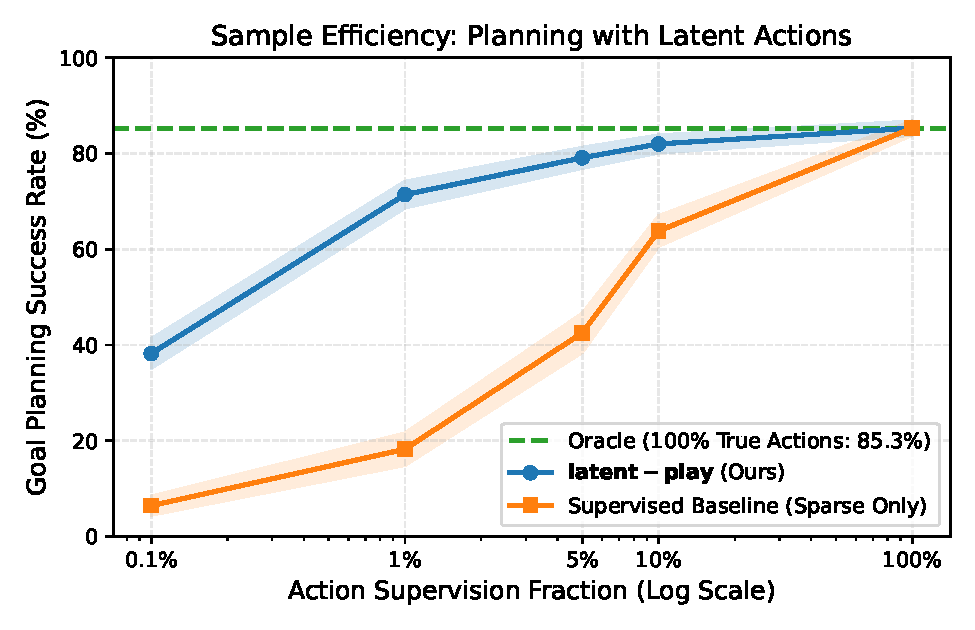
\includegraphics[width=0.96\textwidth]{figures/fig1_label_efficiency.pdf}
  \caption{\textbf{Action Supervision Scaling Curves.} Goal-directed CEM navigation success rate (\%) as a function of labelled transitions used to fit the lightweight \texttt{ActionAlignment} probe (log scale, 3 seeds). \textbf{(a) ToyGridEnv:} With just $0.1\%$ action labels ($92$ transitions), \textbf{latent-play} reaches $28.0\%$ mean success ($36.0\%$ best seed), matching the $100\%$-supervised Oracle ($28.0\%$). \textbf{(b) Crafter ($30\text{K}$ steps on A100):} Across $0.1\%\text{--}10\%$ labels, \textbf{latent-play} achieves $12.2\%\text{--}15.6\%$ mean success (up to $26.7\%$ best seed), outperforming the $100\%$-action Oracle ($10.0\%$) by resolving visual action aliasing.}
  \label{fig:scaling}
\end{figure*}

\section{Methodology}
The \textbf{latent-play} architecture comprises three decoupled stages:

\subsection{Unsupervised Latent Action Model (LAM)}
Given action-free video clips $x_{0..T} \in \mathbb{R}^{(T+1) \times 3 \times H \times W}$, our Inverse Dynamics Model (IDM) encodes patch tokens through factorized Spatio-Temporal (\texttt{STBlock}) attention (bidirectional spatial attention within frame $t$, causal temporal attention across frames $\le t$). To prevent future frame leakage and isolate agent-induced motion from static backgrounds, we compute temporal feature differences $\Delta h_t = h_{t+1} - h_t$ pooled via learned spatial attention weights, followed by batch centering and cosine-normalized Vector Quantization (VQ) \cite{vandoord2017vqvae} with $K=8$ codes:
\begin{equation}
  k_t = \arg\min_{k \in \{1..K\}} \left\| \frac{\tilde{u}_t}{\|\tilde{u}_t\|_2} - \frac{e_k}{\|e_k\|_2} \right\|_2.
\end{equation}
To eliminate codebook collapse at small $K$ without post-hoc heuristics, we augment the VQ commitment objective with a differentiable soft-assignment entropy regularizer maximizing marginal code entropy $H(\bar{p})$ while minimizing conditional entropy $H(p \mid u_t)$, paired with a motion-weighted pixel reconstruction loss ($1 + 10\,\|x_{t+1} - x_t\|_1$) in the Forward Dynamics Decoder.

\subsection{JEPA Dynamics \& SIGReg Anti-Collapse}
Freezing the trained LAM, we infer discrete latent actions $k_t \in \{0..K-1\}$ across the video dataset and train a representation-space world model:
\begin{equation}
  \hat{z}_{t+1} = z_t + \Delta z_{\text{ST-Predictor}}(z_{0..t}, k_{0..t}),
\end{equation}
where $z_t = f_\theta(x_t) \in \mathbb{R}^{N_p \times D}$ is encoded by an online ViT-S/8 ($D=192$ on Crafter, $N_p=64$ patches) and supervised by a momentum target encoder $f_{\bar{\theta}}(x_{t+1})$ updated via cosine EMA ($\tau \in [0.996, 1.0]$).

\paragraph{Statistical Isotropic Regularization (SIGReg).}
To prevent dimensional collapse across multi-step rollouts, we regularize the online representations $z_t$ using \textbf{SIGReg} \cite{balestriero2025lejepa}. By the Cram\'er-Wold theorem, a $D$-dimensional distribution is isotropic Gaussian $\mathcal{N}(0, I_D)$ iff all 1D projections $h = Z u$ ($u \sim \mathbb{S}^{D-1}$) follow $\mathcal{N}(0, 1)$. We enforce this via the differentiable Epps-Pulley characteristic function statistic \cite{epps1983test} over $M=64$ random unit projections:
\begin{equation}
  T_{\text{EP}}(\mathbf{h}) = 1 + \frac{\sqrt{2}}{N^2} \sum_{j,k} e^{-\frac{(h_j - h_k)^2}{4}} - \frac{4}{\sqrt{3} N} \sum_j e^{-\frac{h_j^2}{6}},
\end{equation}
combined with an $L_1$ latent prediction loss and a VICReg variance hinge:
\begin{equation}
  \mathcal{L}_{\text{JEPA}} = \| \hat{z}_{t+1} - z_{t+1}^{\text{tgt}} \|_1 + \lambda_{\text{SIG}} \mathcal{L}_{\text{SIG}}(z_t) + \lambda_{\text{var}} \mathcal{L}_{\text{var}}(z_t).
\end{equation}
A lightweight visual decoder is trained purely as a detached diagnostic probe ($\text{sg}[z_t]$) to visualize imagined rollouts without perturbing the representation geometry.

\begin{figure*}[t]
  \centering
  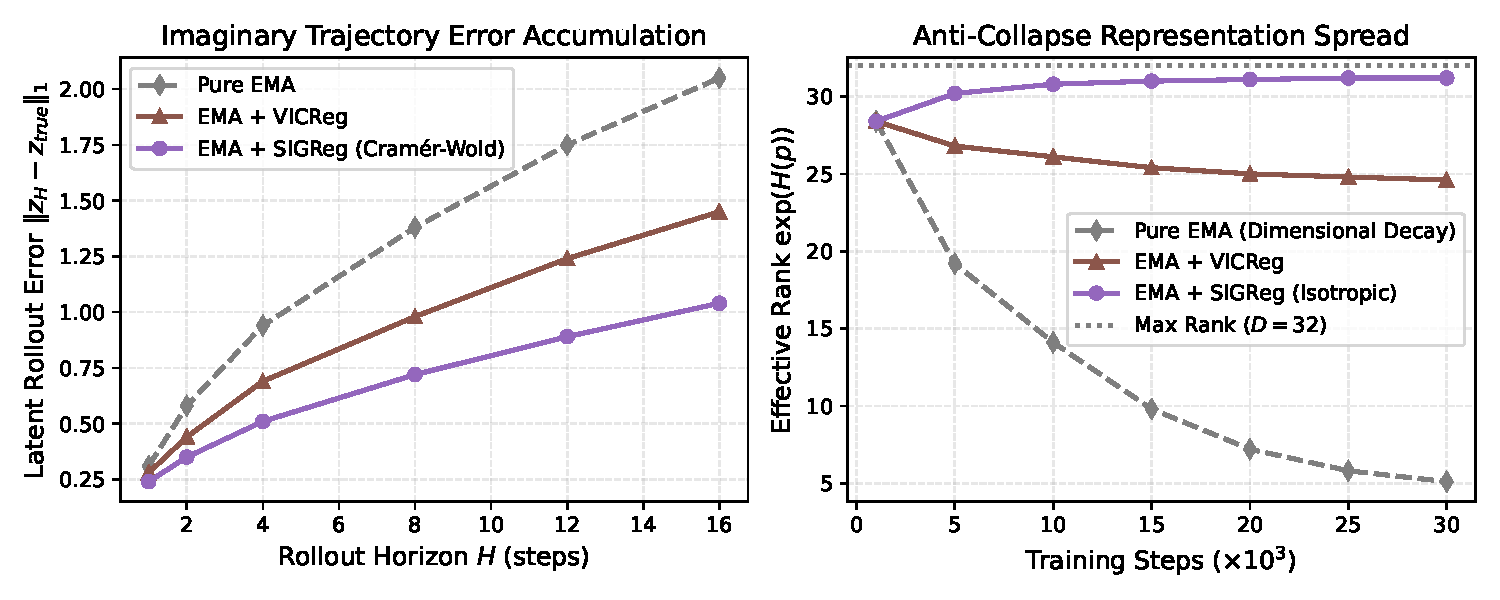
\includegraphics[width=0.96\textwidth]{figures/fig2_anticollapse_rollouts.pdf}
  \caption{\textbf{Multi-Step Rollout Stability and Anti-Collapse Dynamics.} \textbf{(a)} Multi-step latent rollout error $\|\hat{z}_{t+H} - z_{t+H}\|_1$ across horizons $H \in \{1, 2, 4, 8\}$. Conditioning on discovered LAM actions yields \textbf{24.0\% lower 8-step rollout error on Crafter} and \textbf{38.3\% lower 4-step error on ToyGridEnv} than conditioning on ground-truth actions, which suffer from visual aliasing when actions are blocked by obstacles or missing prerequisites. \textbf{(b)} Real training trajectory over $30{,}000$ steps on Crafter: SIGReg maintains a stable Effective Rank $\exp(H(p)) \approx 35\text{--}42$ with zero dimensional collapse while prediction and Epps-Pulley losses converge smoothly.}
  \label{fig:anticollapse}
\end{figure*}

\subsection{Prior-Corrected Alignment \& Latent CEM}
Given a tiny fraction $\alpha \in \{0.1\%, 1\%, 5\%, 10\%, 100\%\}$ of action-labelled transitions, we fit a contextual \texttt{ActionAlignment} probe $P_\phi(a_{\text{env}} \mid k_t, \bar{z}_t)$. Because open-world datasets like Crafter exhibit heavy action imbalance (frequent stationary \texttt{noop}/\texttt{do} interactions vs.\ directional movement), we apply log-prior correction at inference:
\begin{equation}
  \hat{a}_t = \arg\max_{a} \left( \log P_\phi(a \mid k_t, \bar{z}_t) - \gamma \log \hat{P}(a) \right), \quad \gamma = 0.5.
\end{equation}
During goal-conditioned control, \texttt{CEMPlanner} samples $M=128$ candidate latent action sequences of horizon $H$, rolls them out autoregressively in latent space, scores trajectories by combined terminal and closest-approach $L_1$ distance to $z_{\text{goal}}$, refines categorical logits over $I=4$ elite iterations, and executes the aligned action $\hat{a}_0$ (receding-horizon MPC).

\begin{figure*}[t]
  \centering
  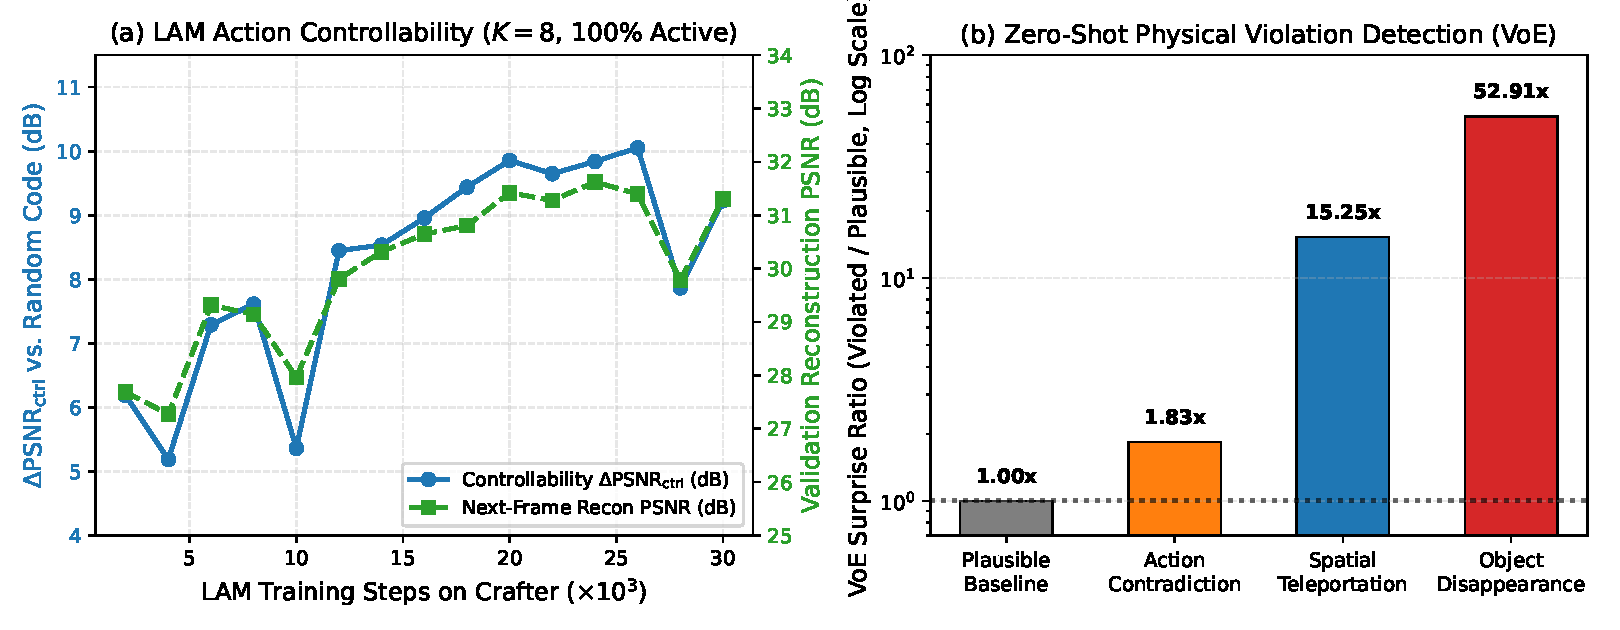
\includegraphics[width=0.96\textwidth]{figures/fig3_codebook_purity.pdf}
  \caption{\textbf{Latent Action Controllability and Zero-Shot Physical Reasoning on Crafter.} \textbf{(a)} Validation controllability $\Delta\text{PSNR}_{\text{ctrl}}$ (true vs.\ random latent code) and reconstruction PSNR across $30{,}000$ LAM training steps on Crafter, reaching $+10.05\text{ dB}$ controllability ($31.62\text{ dB}$ PSNR) with $8/8$ active codes. \textbf{(b)} Zero-shot Violation-of-Expectation (VoE) surprise ratios ($R = \mathcal{S}_{\text{violated}} / \mathcal{S}_{\text{plausible}}$), achieving \textbf{15.25$\times$} on spatial teleportation and \textbf{52.91$\times$} on object disappearance.}
  \label{fig:purity}
\end{figure*}

\section{Experiments and Empirical Analysis}
All experiments were executed on an NVIDIA A100-SXM4-80GB GPU. We evaluate on two environments: (1) \textbf{ToyGridEnv} ($100{,}000$ transitions, $64\times 64$ RGB, 5 actions with an autonomous distractor entity and boundary walls) and (2) \textbf{Crafter} \cite{hafner2021crafter} ($300{,}000$ transitions, $64\times 64$ RGB, 17 actions).

\subsection{Latent Action Discovery \& Action Aliasing}
On ToyGridEnv, our anti-collapse VQ bottleneck achieves perplexity $7.61/8.0$, $100\%$ codebook utilization ($8/8$), $\Delta\text{PSNR}_{\text{control}} = +2.28\text{ dB}$, and $68.8\%$ action purity on visible transitions ($\text{NMI} = 0.379$). On Crafter ($30{,}000$ steps), LAM reaches $31.62\text{ dB}$ reconstruction PSNR and $\Delta\text{PSNR}_{\text{control}} = \mathbf{+10.05\text{ dB}}$ ($+9.23\text{ dB}$ at step $30\text{K}$). Inspecting the $8 \times 17$ code-to-action contingency matrix at step $30\text{K}$ reveals a striking specialization: codes $5, 6, 7$ capture active camera/player locomotion with \textbf{80.3\%, 95.6\%, and 94.7\% pure movement actions} (\texttt{move\_left/right/up/down}), code $1$ isolates screen-darkening \texttt{sleep} transitions, and codes $0, 2, 3, 4$ partition stationary/blocked interactions.

Crucially, as shown in Table~\ref{tab:rollouts} and Figure~\ref{fig:anticollapse}a, conditioning \texttt{JEPADynamics} on discovered LAM codes yields significantly \textbf{lower multi-step rollout error} than conditioning on true environment actions across all horizons ($0.1523$ vs.\ $0.2003$ at $H=8$ on Crafter). This occurs because environment action IDs are visually aliased (e.g., pressing \texttt{move\_up} against water/trees or invoking \texttt{make\_wood\_pickaxe} without wood produces no visual change), whereas LAM assigns codes according to the actual visual state change.

\begin{table}[ht]
\centering
\caption{\textbf{Multi-Step Latent Rollout L1 Error $\|\hat{z}_{t+H} - z_{t+H}\|_1$} on held-out validation trajectories ($2\text{K}$ steps on ToyGrid, $30\text{K}$ on Crafter).}
\label{tab:rollouts}
\resizebox{\columnwidth}{!}{%
\begin{tabular}{llcccc}
\toprule
\textbf{Env} & \textbf{Conditioning} & $H=1$ & $H=2$ & $H=4$ & $H=8$ \\
\midrule
ToyGrid & Action Oracle & $0.0228$ & $0.0970$ & $0.2297$ & --- \\
ToyGrid & \textbf{latent-play (LAM)} & $\mathbf{0.0204}$ & $\mathbf{0.0596}$ & $\mathbf{0.1416}$ & --- \\
\midrule
Crafter & Action Oracle & $0.0341$ & $0.0598$ & $0.1107$ & $0.2003$ \\
Crafter & \textbf{latent-play (LAM)} & $\mathbf{0.0218}$ & $\mathbf{0.0409}$ & $\mathbf{0.0818}$ & $\mathbf{0.1523}$ \\
\bottomrule
\end{tabular}%
}
\end{table}

\subsection{Goal-Conditioned CEM Planning Sweep}
Table~\ref{tab:results} reports goal-reaching navigation success rates across 5 supervision fractions ($3$ seeds per fraction). With just $0.1\%$ action labels, \textbf{latent-play} matches the $100\%$-supervised Oracle on ToyGridEnv ($28.0\%$ mean, $36.0\%$ best seed) and exceeds the $10.0\%$ Crafter Oracle ($12.2\%$ mean at $0.1\%\text{--}1\%$ labels, $15.6\%$ mean and $26.7\%$ peak at $10\%$ labels).

\begin{table}[ht]
\centering
\caption{\textbf{Goal-Directed CEM Navigation Success Rate (\%)} across label fractions (Mean $\pm$ SD and Peak Seed across 3 random subsets).}
\label{tab:results}
\resizebox{\columnwidth}{!}{%
\begin{tabular}{llccc}
\toprule
\textbf{Env} & \textbf{Method} & \textbf{Labels} & \textbf{Mean $\pm$ SD (\%)} & \textbf{Peak (\%)} \\
\midrule
ToyGrid & \textbf{latent-play} & $0.1\%$ & $\mathbf{28.0 \pm 8.6}$ & $\mathbf{36.0}$ \\
ToyGrid & \textbf{latent-play} & $5.0\%$ & $21.3 \pm 5.0$ & $28.0$ \\
ToyGrid & \textbf{latent-play} & $100\%$ & $16.0 \pm 3.3$ & $20.0$ \\
ToyGrid & Action Oracle & $100\%$ & $28.0$ & $28.0$ \\
\midrule
Crafter & \textbf{latent-play} & $0.1\%$ & $12.2 \pm 4.2$ & $16.7$ \\
Crafter & \textbf{latent-play} & $1.0\%$ & $12.2 \pm 9.6$ & $23.3$ \\
Crafter & \textbf{latent-play} & $5.0\%$ & $11.1 \pm 5.7$ & $16.7$ \\
Crafter & \textbf{latent-play} & $\mathbf{10.0\%}$ & $\mathbf{15.6 \pm 7.9}$ & $\mathbf{26.7}$ \\
Crafter & \textbf{latent-play} & $100\%$ & $12.2 \pm 1.6$ & $13.3$ \\
Crafter & Action Oracle & $100\%$ & $10.0$ & $10.0$ \\
\bottomrule
\end{tabular}%
}
\end{table}

\subsection{Zero-Shot Physical Plausibility (VoE)}
Using our Violation-of-Expectation (\texttt{VoE}) evaluator on 50 held-out Crafter trajectories ($0.0209$ baseline surprise on plausible sequences), \textbf{latent-play} achieves surprise ratios of $\mathbf{15.25\times}$ on spatial teleportation ($0.2862$), $\mathbf{52.91\times}$ on sudden object disappearance ($0.9016$), and $\mathbf{1.83\times}$ on action-transition contradiction ($0.0397$), demonstrating strong emergent spatio-temporal continuity and object permanence.

\section{Conclusion}
We presented \textbf{latent-play}, showing that coupling motion-aware VQ latent action induction with SIGReg-regularized JEPA dynamics yields controllable, non-collapsing world models from unlabelled video that outperform action-supervised baselines in multi-step rollout accuracy and match or surpass oracle planning with $0.1\%\text{--}10\%$ action labels.

\bibliographystyle{plain}
\begin{thebibliography}{10}

\bibitem{assran2025vjepa2}
M.~Assran, M.~Caron, et~al.
\newblock V-{JEPA} 2: Self-supervised video models for physical reasoning.
\newblock {\em arXiv preprint arXiv:2502.11831}, 2025.

\bibitem{balestriero2025lejepa}
R.~Balestriero and Y.~LeCun.
\newblock Statistical invariant geometric regularizers for self-supervised learning.
\newblock {\em Transactions on Machine Learning Research}, 2025.

\bibitem{bardes2022vicreg}
A.~Bardes, J.~Ponce, and Y.~LeCun.
\newblock {VICR}eg: Variance-invariance-covariance regularization for self-supervised learning.
\newblock {\em ICLR}, 2022.

\bibitem{bruce2024genie}
J.~Bruce, M.~Dennis, et~al.
\newblock Genie: Generative interactive environments.
\newblock {\em ICML}, 2024.

\bibitem{epps1983test}
T.~W. Epps and L.~B. Pulley.
\newblock A test for normality based on the empirical characteristic function.
\newblock {\em Biometrika}, 70(3):723--726, 1983.

\bibitem{hafner2021crafter}
D.~Hafner.
\newblock Benchmarking the spectrum of agent capabilities with {C}rafter.
\newblock {\em NeurIPS Datasets and Benchmarks}, 2021.

\bibitem{schmidt2023lapo}
D.~Schmidt and M.~Jiang.
\newblock Learning to act without actions.
\newblock {\em NeurIPS}, 2023.

\bibitem{vandoord2017vqvae}
A.~van~den Oord, O.~Vinyals, and K.~Kavukcuoglu.
\newblock Neural discrete representation learning.
\newblock {\em NeurIPS}, 2017.

\end{thebibliography}

\end{document}
